\newgeometry{margin=0in}
\begin{figure}[p]
    \centering
    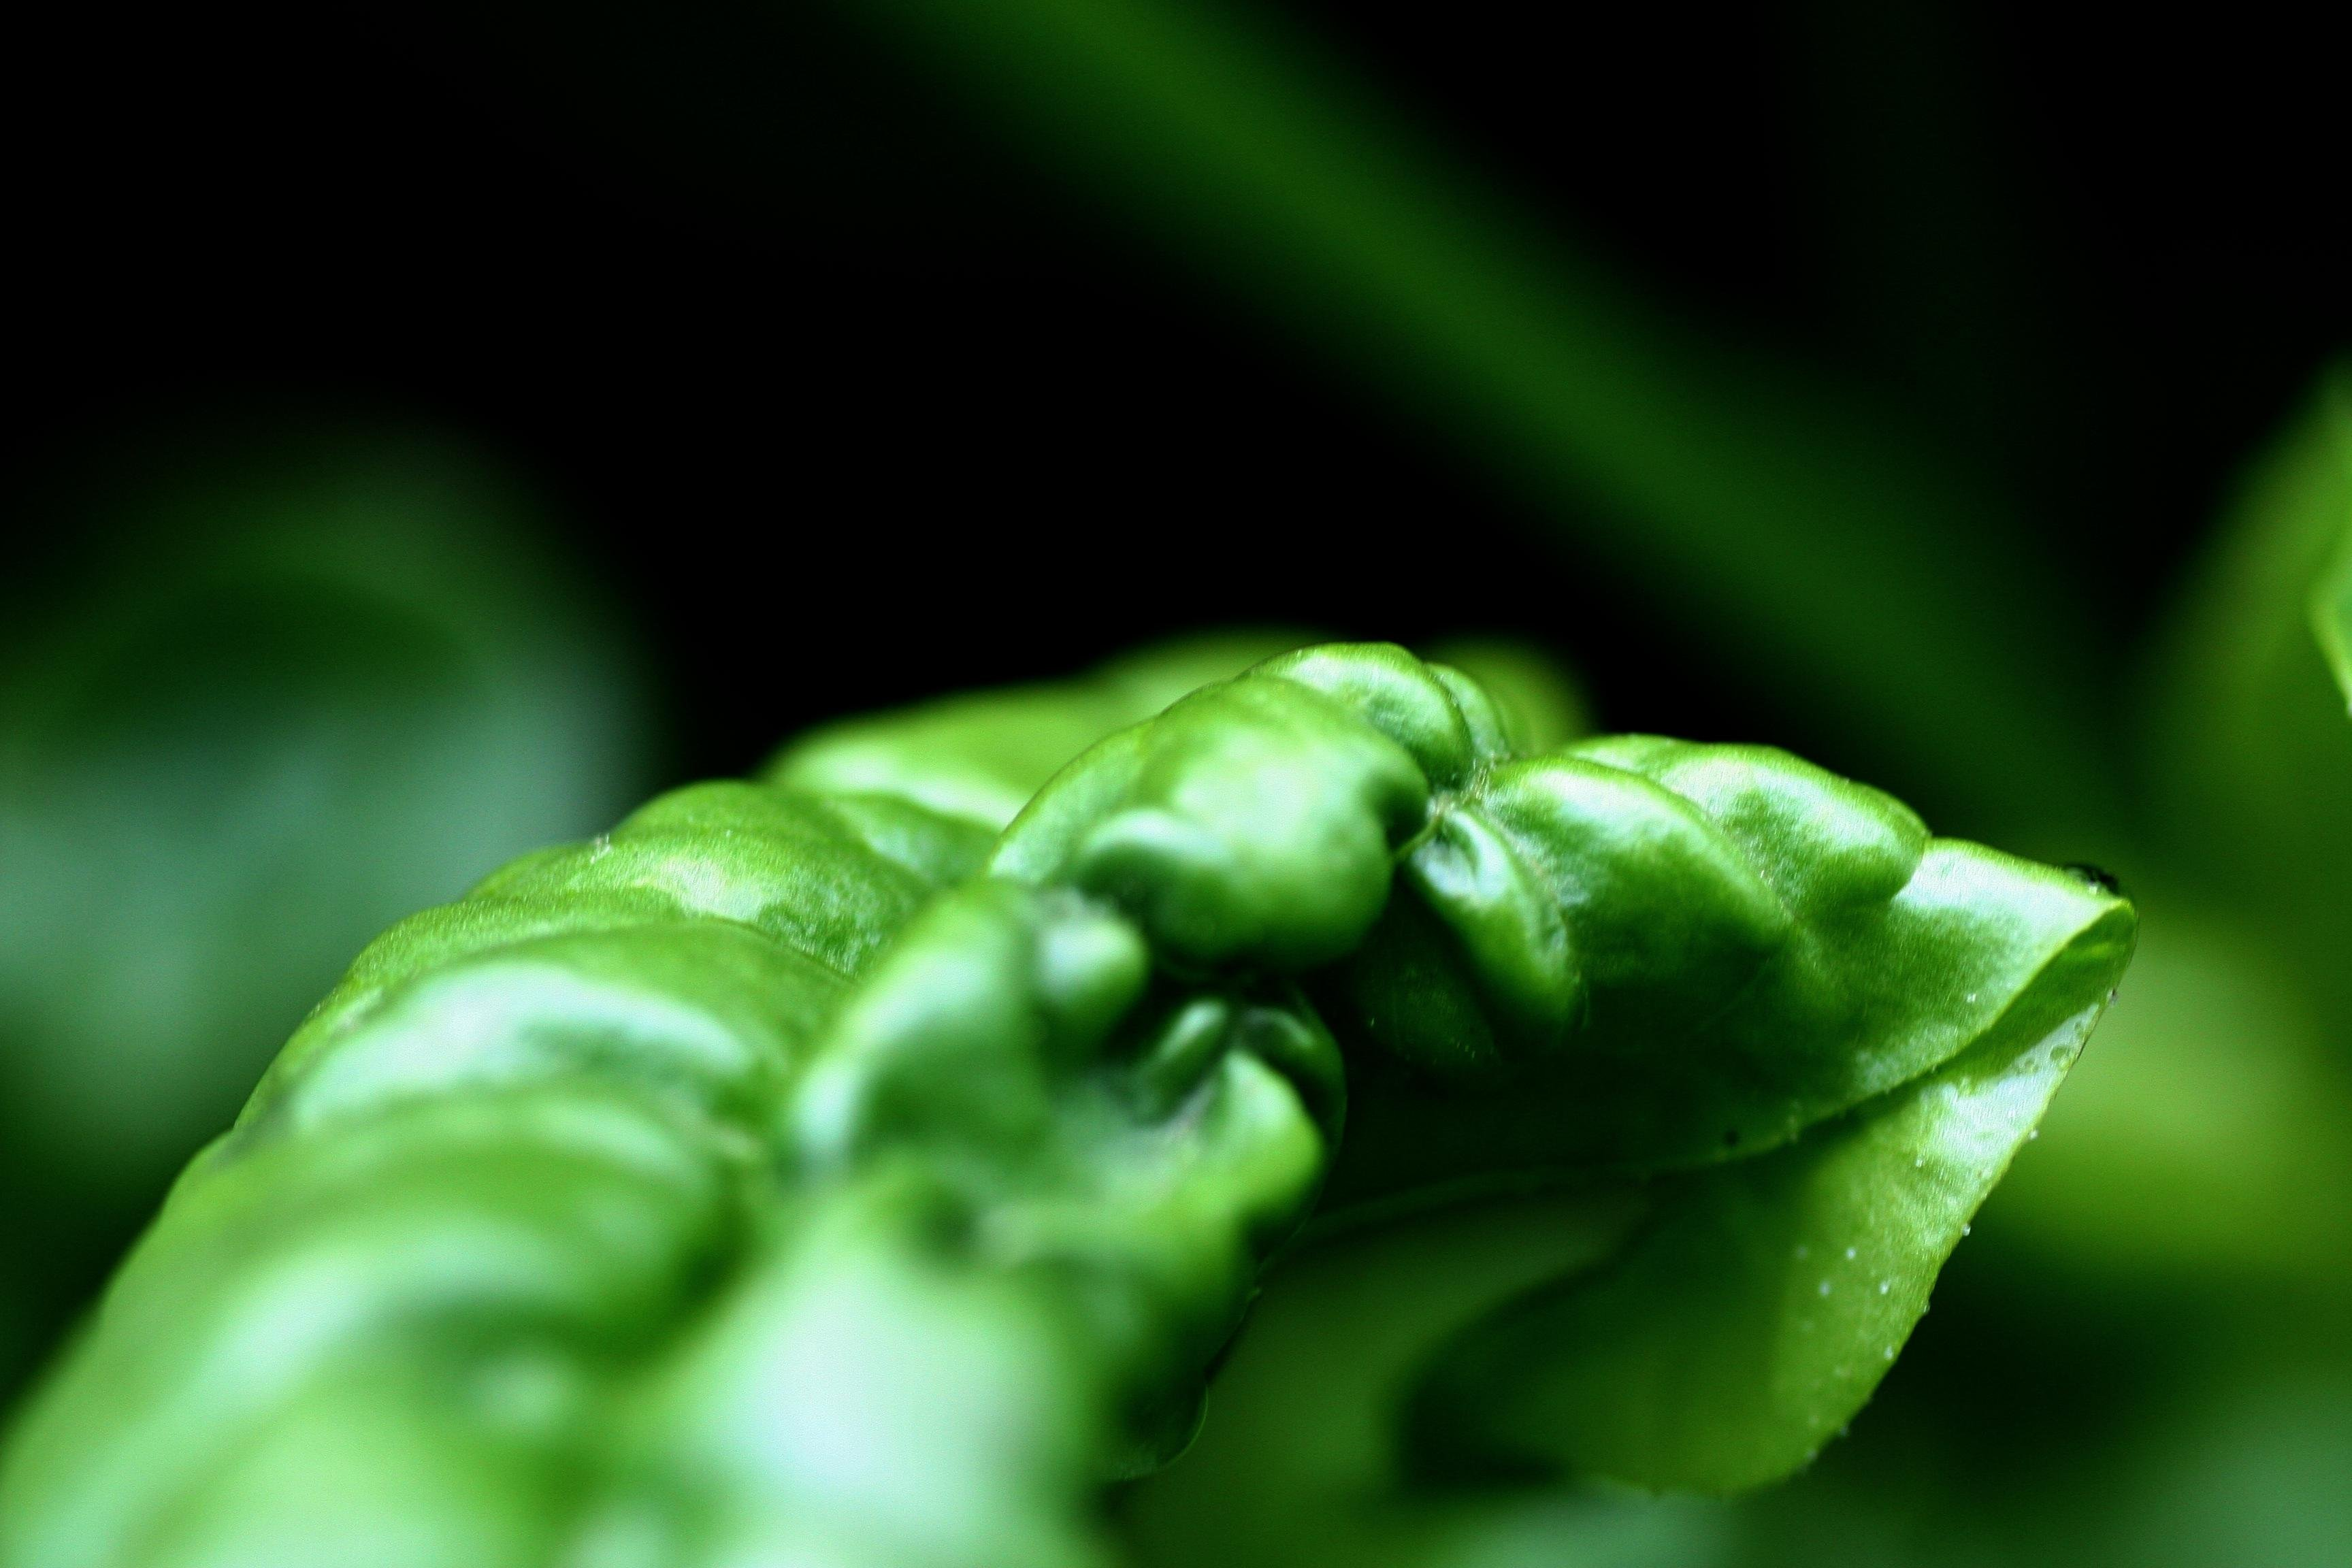
\includegraphics[width=\paperwidth,height=\paperheight]{spinach.jpg}
    \caption{Fresh Spinach}
\end{figure}
\restoregeometry
\clearpage

\section{Anne's Spinach Salad}
\begin{multicols*}{3}

\begin{quote}
    This recipe is from my Aunt Anne, who swears that she always used romaine lettuce instead of spinach.
\end{quote}

\begin{tabular}{r@{ }l}
    2 & eggs \\
\end{tabular}

Boil eggs, cool, shell and slice into rings.

\begin{tabular}{r@{ }l}
    10 & strips bacon \\
\end{tabular}

Separate strips onto aluminum foil in a baking sheet, and bake for 15 minutes at 425. Pat dry and chop into small pieces.

\begin{tabular}{r@{ }l}
    \sfrac{1}{2} & cup olive oil \\
    \sfrac{3}{4} & can anchovies in oil \\
               2 & tablespoons balsamic \\
               2 & tablespoons lemon juice \\
               1 & garlic clove \\
    \sfrac{1}{2} & teaspoon thyme \\
    \sfrac{1}{4} & teaspoon \\
                 & sugar \\
                 & oregano \\
                 & mustard powder \\
                 & onion salt \\
                 & paprika \\
\end{tabular}

Discard the oil in the can and use only the anchovies. Liquefy all  ingredients in a blender.

\begin{tabular}{r@{ }l}
    1 & package spinach \\
      & pre-sliced mushrooms \\
\end{tabular}

Combine eggs, bacon and dressing in a large mixing bowl.

\begin{quote}
The dressing can keep at least overnight.

To shell eggs easily, run under cold water, shaking pan to smash shells. The water will seep in. In 10 minutes, the shells will come off easily.

Leftover spinach can be saved, but be sure to reseal it in the original packaging, which is specially designed to breath. Spinach or lettuce saved in regular plastic will rot in a few days.

If you want to chop bacon very fine, freeze it for 10 minutes first.
\end{quote}

\end{multicols*}

\clearpage
